\documentclass[11pt]{article}
\usepackage[textwidth=18.0cm, textheight=23.0cm, top=2.0cm]{geometry}
\usepackage{pst-all}
\usepackage{amssymb}
\usepackage{tikz}
\usepackage{underscore}\begin{document}
\pagestyle{empty}


ClassName: \underline{\textbf{Class_10.2bp-44}}
\par
BinSize: \underline{\textbf{100 × 100}}
\par
ReduceSize: \underline{\textbf{100 × 100}}
\par
TypeNum: \underline{\textbf{100}}
\par
Num: \underline{\textbf{100}}
\par
OutS: \underline{\textbf{180000}}
\par
InS: \underline{\textbf{164869}}
\par
Rate: \underline{\textbf{0.916}}
\par
UB: \underline{\textbf{18}}
\par
LB0: \underline{\textbf{17}}
\par
LB: \underline{\textbf{18}}
\par
LBWithCut: \underline{\textbf{18}}
\par
NodeCut: \underline{\textbf{0}}
\par
ExtendedNodeCnt: \underline{\textbf{1}}
\par
GenNodeCnt: \underline{\textbf{1}}
\par
PrimalNode: \underline{\textbf{0}}
\par
ColumnCount: \underline{\textbf{92}}
\par
TotalCutCount: \underline{\textbf{0}}
\par
RootCutCount: \underline{\textbf{0}}
\par
LPSolverCnt: \underline{\textbf{74}}
\par
PricingSolverCnt: \underline{\textbf{74}}
\par
BranchAndBoundNum: \underline{\textbf{1}}
\par
isOpt: \underline{\textbf{false}}
\par
TimeOnInitSolution: \underline{\textbf{120.020 s}}
\par
TimeOnPrimal: \underline{\textbf{0.000 s}}
\par
TimeOnPricing: \underline{\textbf{4676.959 s}}
\par
TimeOnRmp: \underline{\textbf{0.095 s}}
\par
TotalTime: \underline{\textbf{4797.138 s}}
\par
\newpage


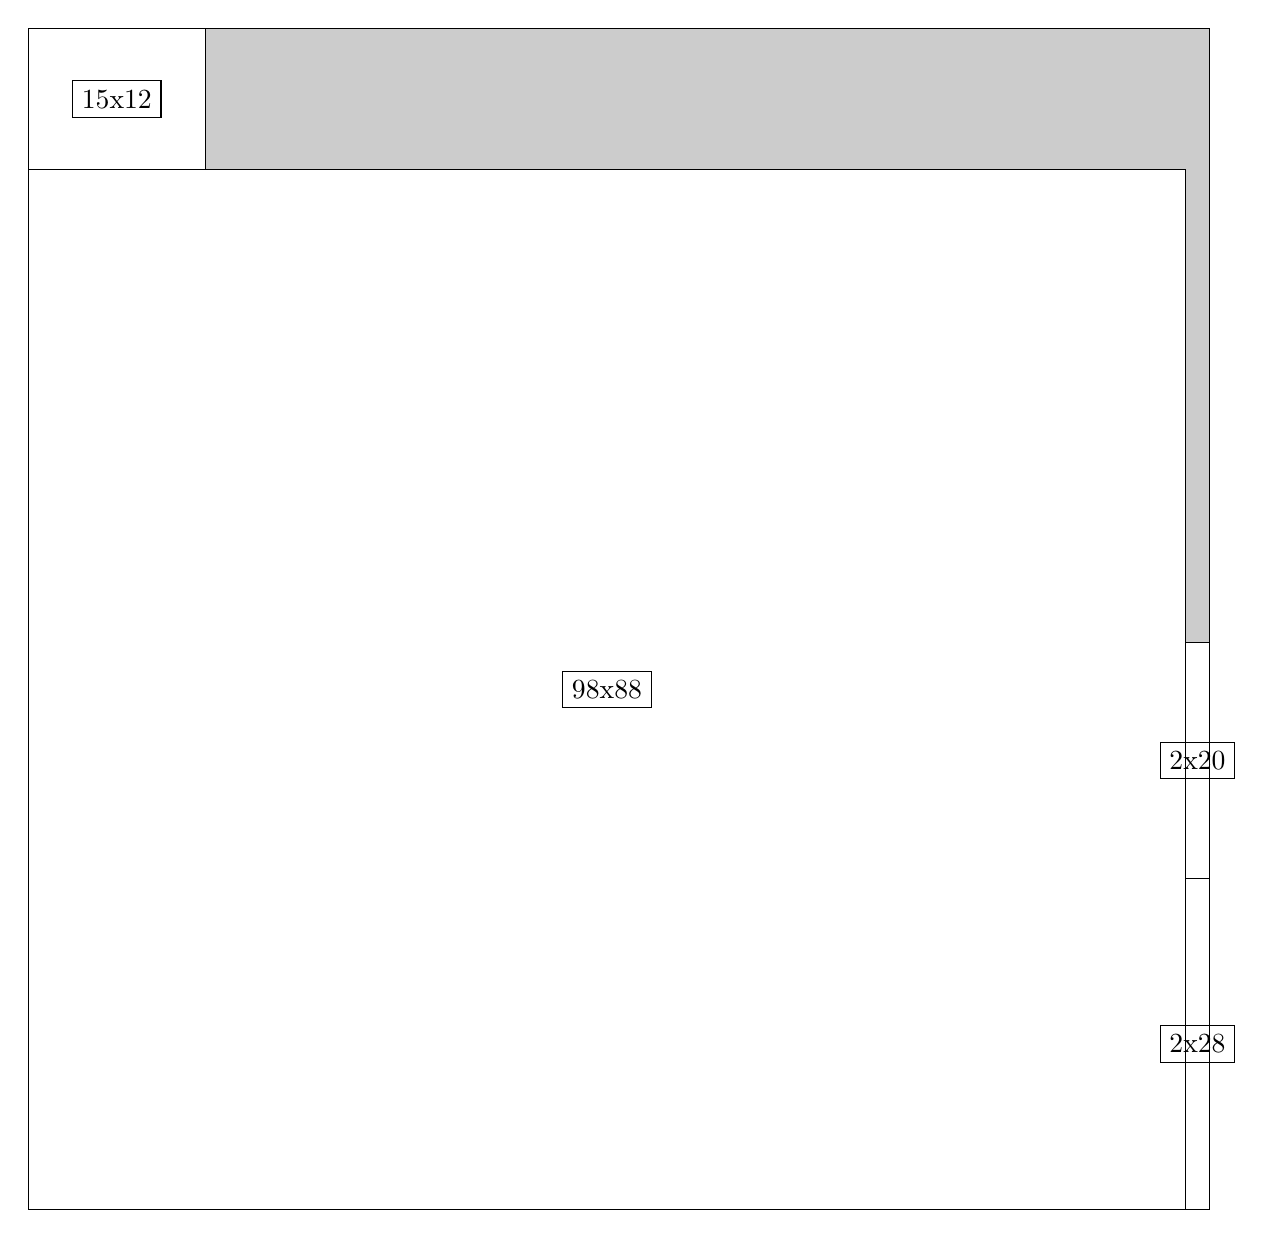
\begin{tikzpicture}[shorten >=1pt,scale=1.0,every node/.style={scale=1.0},->]
\tikzstyle{vertex}=[circle,fill=black!25,minimum size=14pt,inner sep=0pt]
\filldraw[fill=gray!40!white, draw=black] (0,0) rectangle (15.0,15.0);
\foreach \name/\x/\y/\w/\h in {98x88/0.0/0.0/14.7/13.2,15x12/0.0/13.2/2.25/1.7999999999999998,2x28/14.7/0.0/0.3/4.2,2x20/14.7/4.2/0.3/3.0}
\filldraw[fill=white!40!white, draw=black] (\x,\y) rectangle node[draw] (\name) {\name} ++(\w,\h);
\end{tikzpicture}


w =98 , h =88 , x =0 , y =0 , v =8624
\par
w =15 , h =12 , x =0 , y =88 , v =180
\par
w =2 , h =28 , x =98 , y =0 , v =56
\par
w =2 , h =20 , x =98 , y =28 , v =40
\par
\newpage


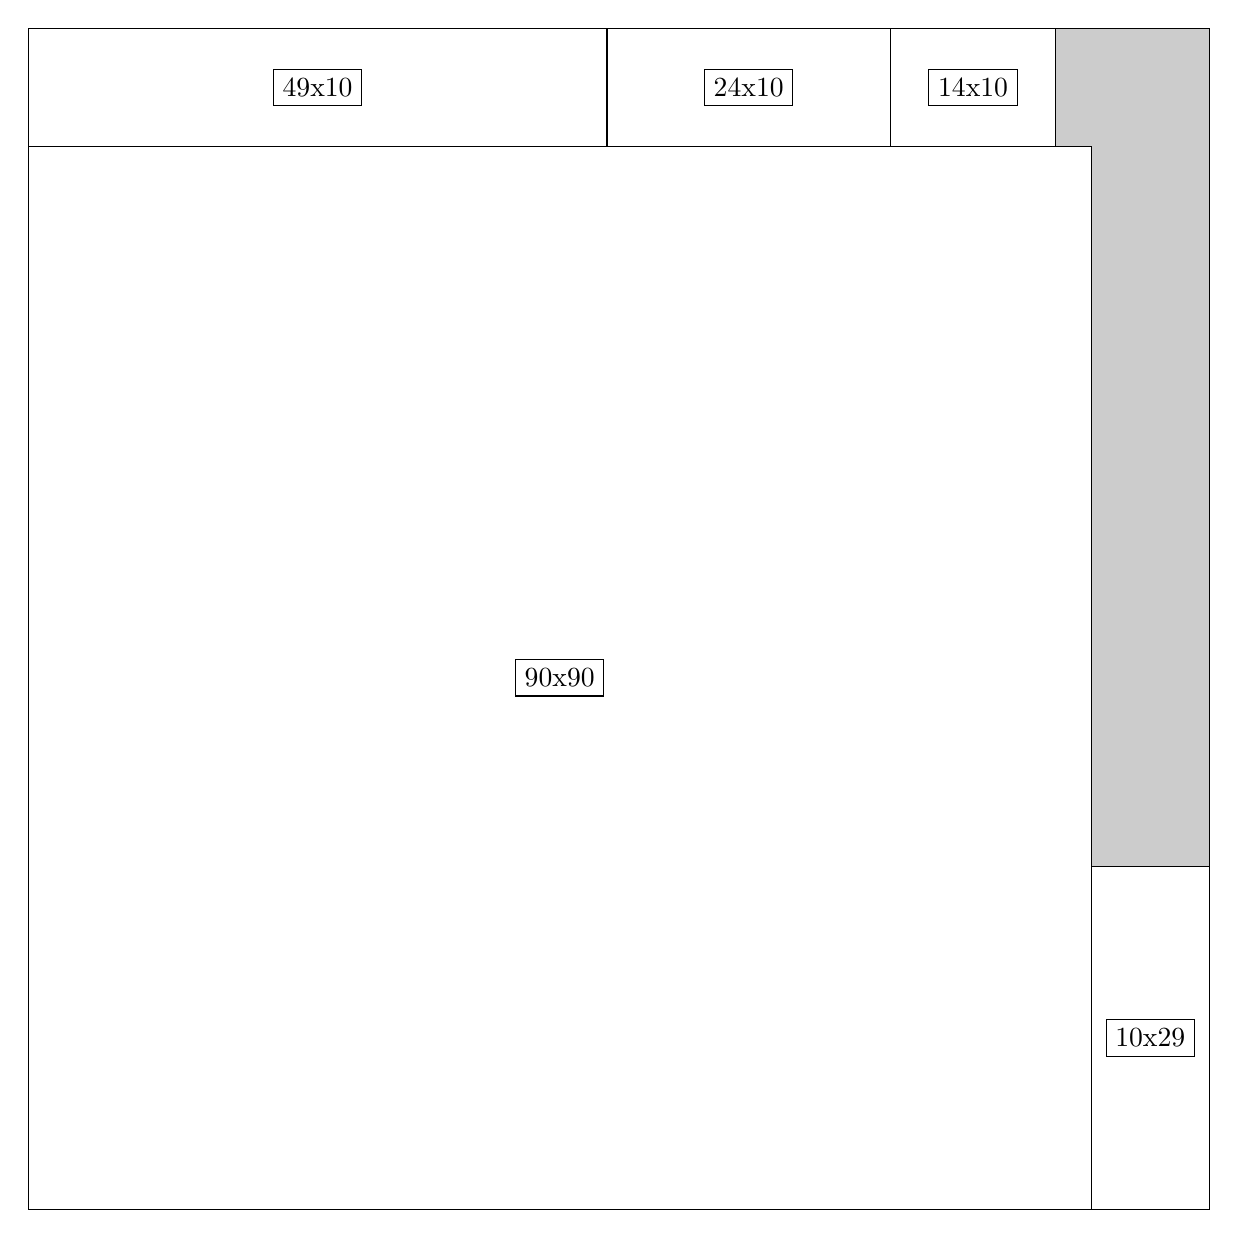
\begin{tikzpicture}[shorten >=1pt,scale=1.0,every node/.style={scale=1.0},->]
\tikzstyle{vertex}=[circle,fill=black!25,minimum size=14pt,inner sep=0pt]
\filldraw[fill=gray!40!white, draw=black] (0,0) rectangle (15.0,15.0);
\foreach \name/\x/\y/\w/\h in {90x90/0.0/0.0/13.5/13.5,49x10/0.0/13.5/7.35/1.5,10x29/13.5/0.0/1.5/4.35,24x10/7.35/13.5/3.5999999999999996/1.5,14x10/10.95/13.5/2.1/1.5}
\filldraw[fill=white!40!white, draw=black] (\x,\y) rectangle node[draw] (\name) {\name} ++(\w,\h);
\end{tikzpicture}


w =90 , h =90 , x =0 , y =0 , v =8100
\par
w =49 , h =10 , x =0 , y =90 , v =490
\par
w =10 , h =29 , x =90 , y =0 , v =290
\par
w =24 , h =10 , x =49 , y =90 , v =240
\par
w =14 , h =10 , x =73 , y =90 , v =140
\par
\newpage


\begin{tikzpicture}[shorten >=1pt,scale=1.0,every node/.style={scale=1.0},->]
\tikzstyle{vertex}=[circle,fill=black!25,minimum size=14pt,inner sep=0pt]
\filldraw[fill=gray!40!white, draw=black] (0,0) rectangle (15.0,15.0);
\foreach \name/\x/\y/\w/\h in {85x92/0.0/0.0/12.75/13.799999999999999,85x8/0.0/13.799999999999999/12.75/1.2,15x43/12.75/0.0/2.25/6.45,15x42/12.75/6.45/2.25/6.3,15x15/12.75/12.75/2.25/2.25}
\filldraw[fill=white!40!white, draw=black] (\x,\y) rectangle node[draw] (\name) {\name} ++(\w,\h);
\end{tikzpicture}


w =85 , h =92 , x =0 , y =0 , v =7820
\par
w =85 , h =8 , x =0 , y =92 , v =680
\par
w =15 , h =43 , x =85 , y =0 , v =645
\par
w =15 , h =42 , x =85 , y =43 , v =630
\par
w =15 , h =15 , x =85 , y =85 , v =225
\par
\newpage


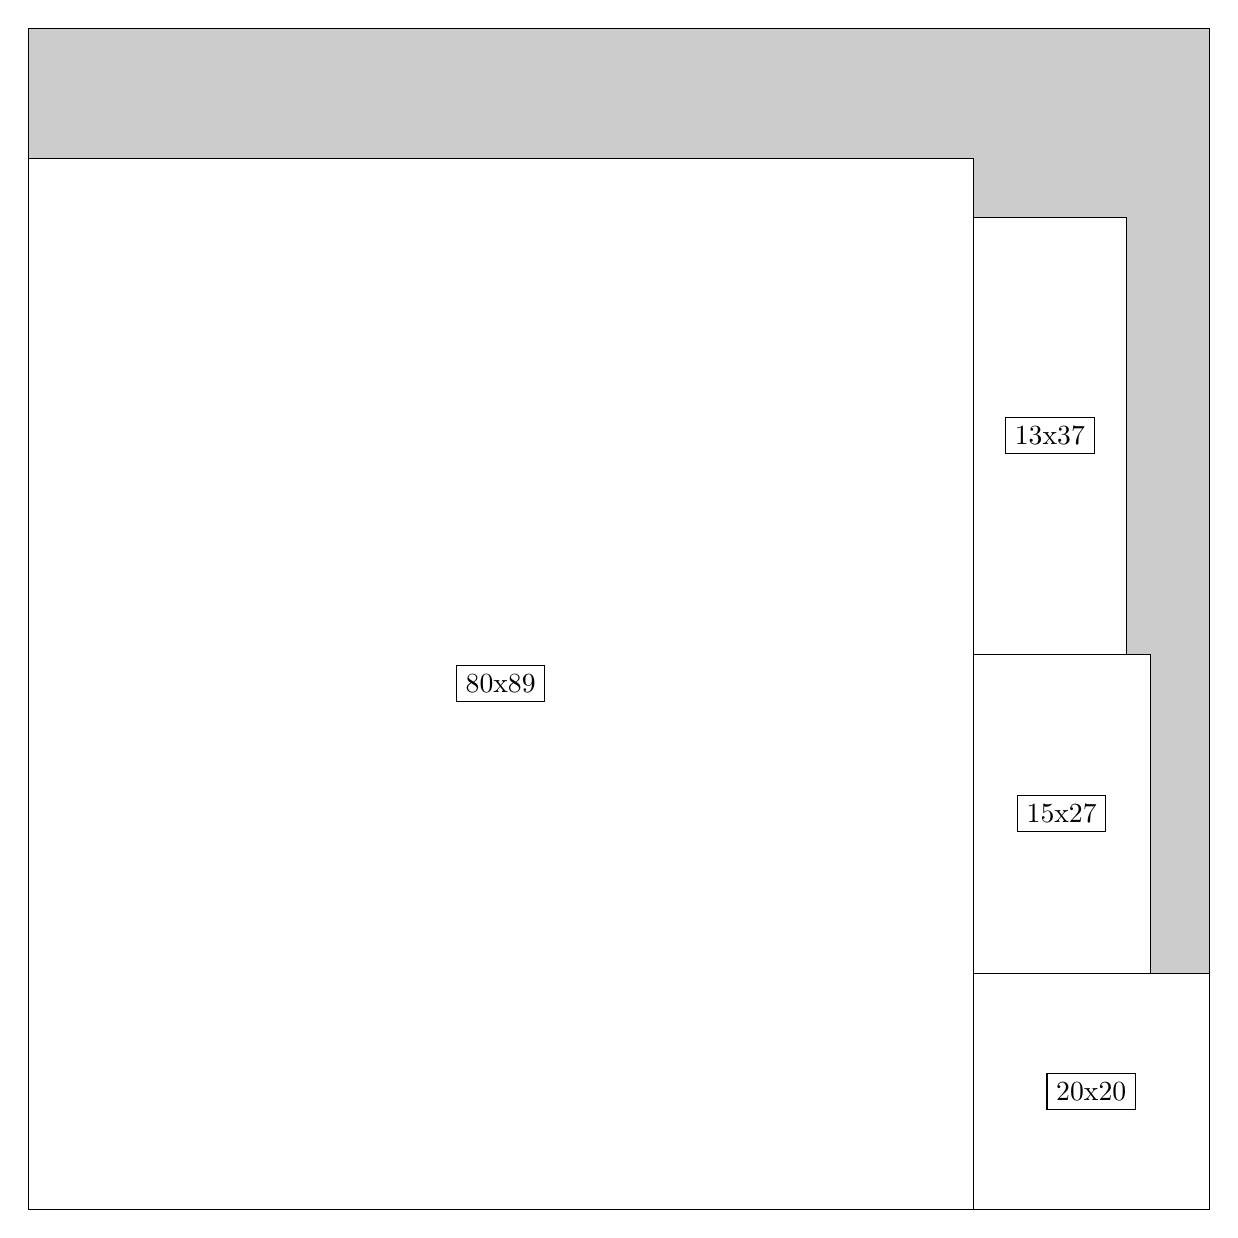
\begin{tikzpicture}[shorten >=1pt,scale=1.0,every node/.style={scale=1.0},->]
\tikzstyle{vertex}=[circle,fill=black!25,minimum size=14pt,inner sep=0pt]
\filldraw[fill=gray!40!white, draw=black] (0,0) rectangle (15.0,15.0);
\foreach \name/\x/\y/\w/\h in {80x89/0.0/0.0/12.0/13.35,13x37/12.0/7.05/1.95/5.55,15x27/12.0/3.0/2.25/4.05,20x20/12.0/0.0/3.0/3.0}
\filldraw[fill=white!40!white, draw=black] (\x,\y) rectangle node[draw] (\name) {\name} ++(\w,\h);
\end{tikzpicture}


w =80 , h =89 , x =0 , y =0 , v =7120
\par
w =13 , h =37 , x =80 , y =47 , v =481
\par
w =15 , h =27 , x =80 , y =20 , v =405
\par
w =20 , h =20 , x =80 , y =0 , v =400
\par
\newpage


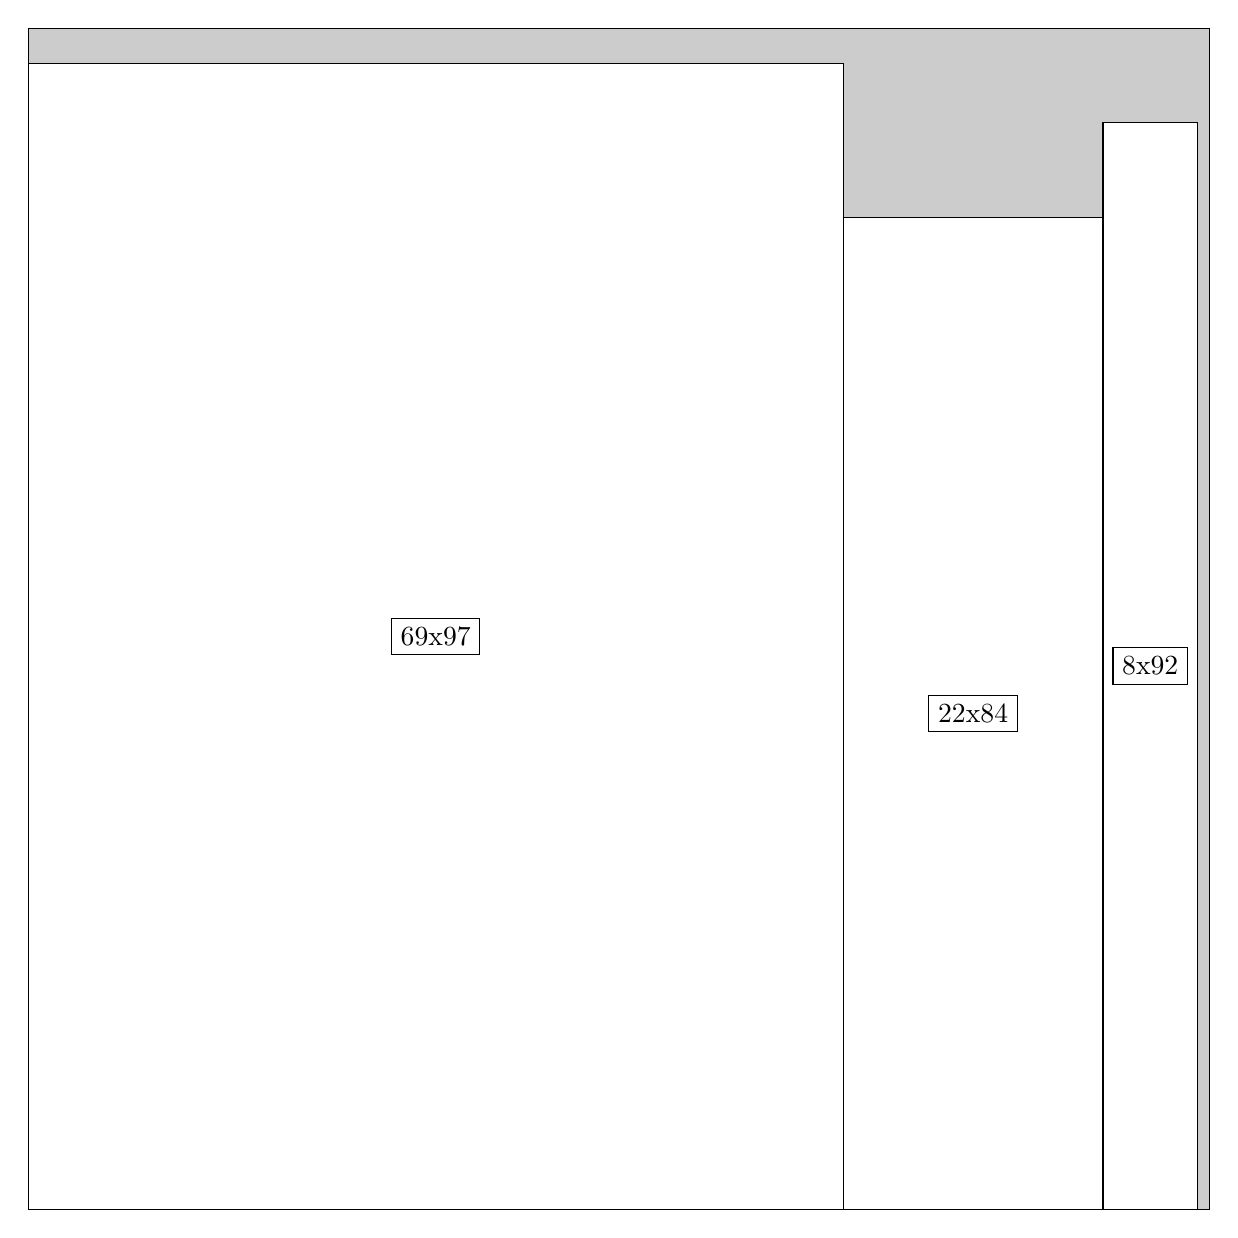
\begin{tikzpicture}[shorten >=1pt,scale=1.0,every node/.style={scale=1.0},->]
\tikzstyle{vertex}=[circle,fill=black!25,minimum size=14pt,inner sep=0pt]
\filldraw[fill=gray!40!white, draw=black] (0,0) rectangle (15.0,15.0);
\foreach \name/\x/\y/\w/\h in {22x84/10.35/0.0/3.3/12.6,69x97/0.0/0.0/10.35/14.549999999999999,8x92/13.65/0.0/1.2/13.799999999999999}
\filldraw[fill=white!40!white, draw=black] (\x,\y) rectangle node[draw] (\name) {\name} ++(\w,\h);
\end{tikzpicture}


w =22 , h =84 , x =69 , y =0 , v =1848
\par
w =69 , h =97 , x =0 , y =0 , v =6693
\par
w =8 , h =92 , x =91 , y =0 , v =736
\par
\newpage


\begin{tikzpicture}[shorten >=1pt,scale=1.0,every node/.style={scale=1.0},->]
\tikzstyle{vertex}=[circle,fill=black!25,minimum size=14pt,inner sep=0pt]
\filldraw[fill=gray!40!white, draw=black] (0,0) rectangle (15.0,15.0);
\foreach \name/\x/\y/\w/\h in {61x98/0.0/0.0/9.15/14.7,39x99/9.15/0.0/5.85/14.85,35x1/9.75/14.85/5.25/0.15,3x1/9.299999999999999/14.85/0.44999999999999996/0.15}
\filldraw[fill=white!40!white, draw=black] (\x,\y) rectangle node[draw] (\name) {\name} ++(\w,\h);
\end{tikzpicture}


w =61 , h =98 , x =0 , y =0 , v =5978
\par
w =39 , h =99 , x =61 , y =0 , v =3861
\par
w =35 , h =1 , x =65 , y =99 , v =35
\par
w =3 , h =1 , x =62 , y =99 , v =3
\par
\newpage


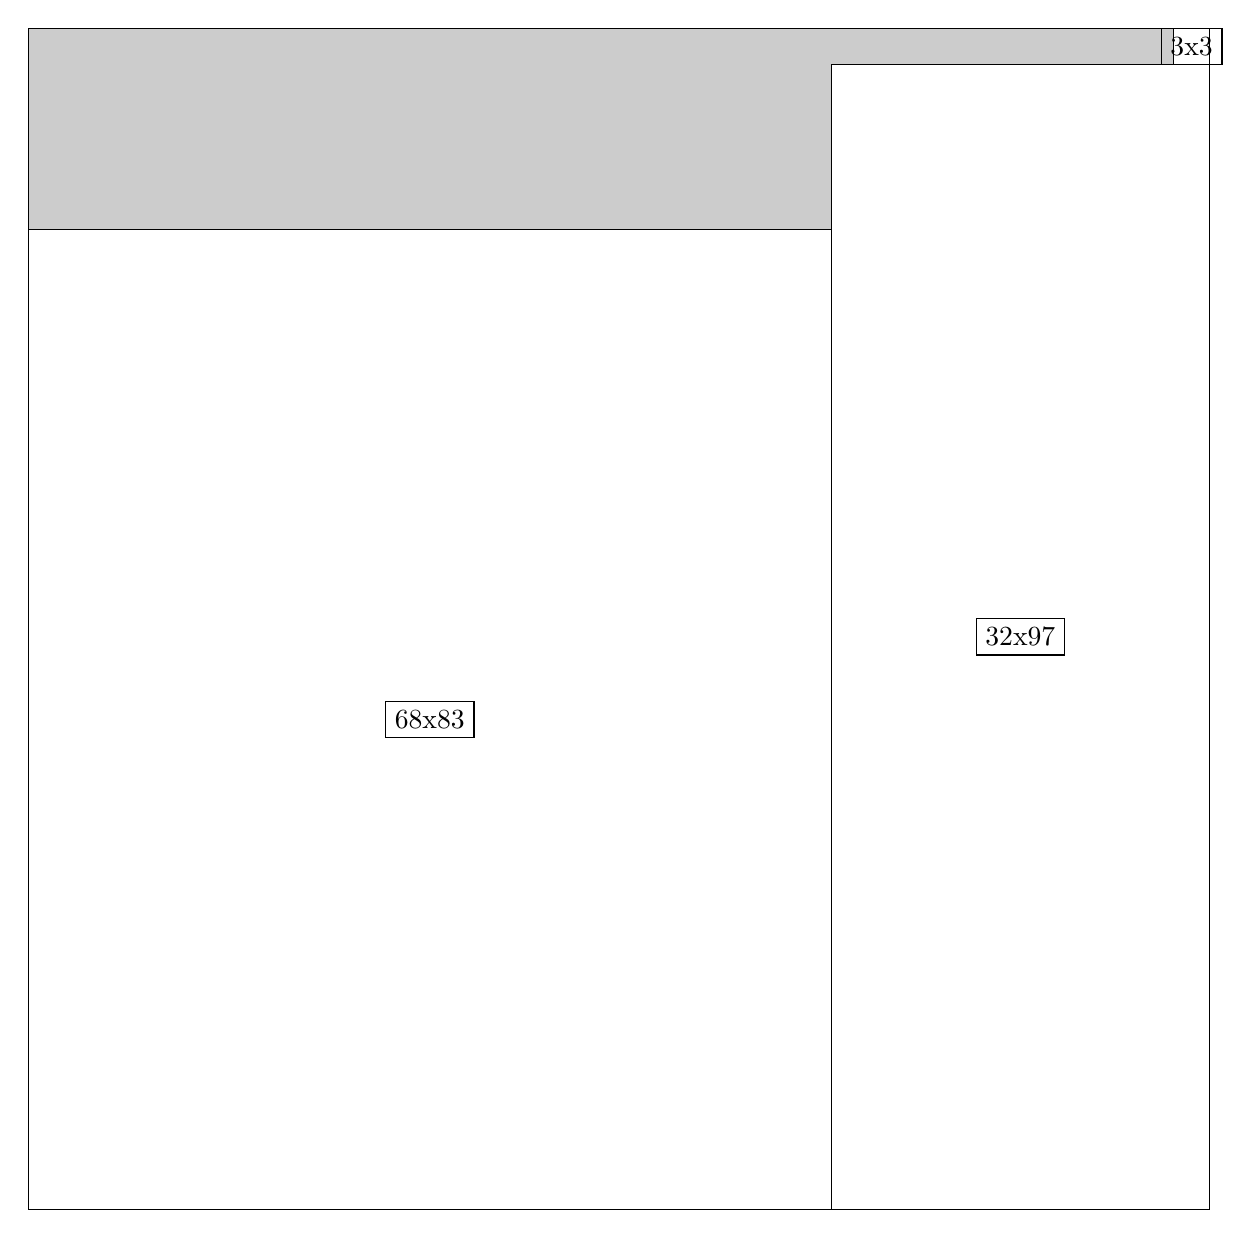
\begin{tikzpicture}[shorten >=1pt,scale=1.0,every node/.style={scale=1.0},->]
\tikzstyle{vertex}=[circle,fill=black!25,minimum size=14pt,inner sep=0pt]
\filldraw[fill=gray!40!white, draw=black] (0,0) rectangle (15.0,15.0);
\foreach \name/\x/\y/\w/\h in {68x83/0.0/0.0/10.2/12.45,32x97/10.2/0.0/4.8/14.549999999999999,3x3/14.549999999999999/14.549999999999999/0.44999999999999996/0.44999999999999996}
\filldraw[fill=white!40!white, draw=black] (\x,\y) rectangle node[draw] (\name) {\name} ++(\w,\h);
\end{tikzpicture}


w =68 , h =83 , x =0 , y =0 , v =5644
\par
w =32 , h =97 , x =68 , y =0 , v =3104
\par
w =3 , h =3 , x =97 , y =97 , v =9
\par
\newpage


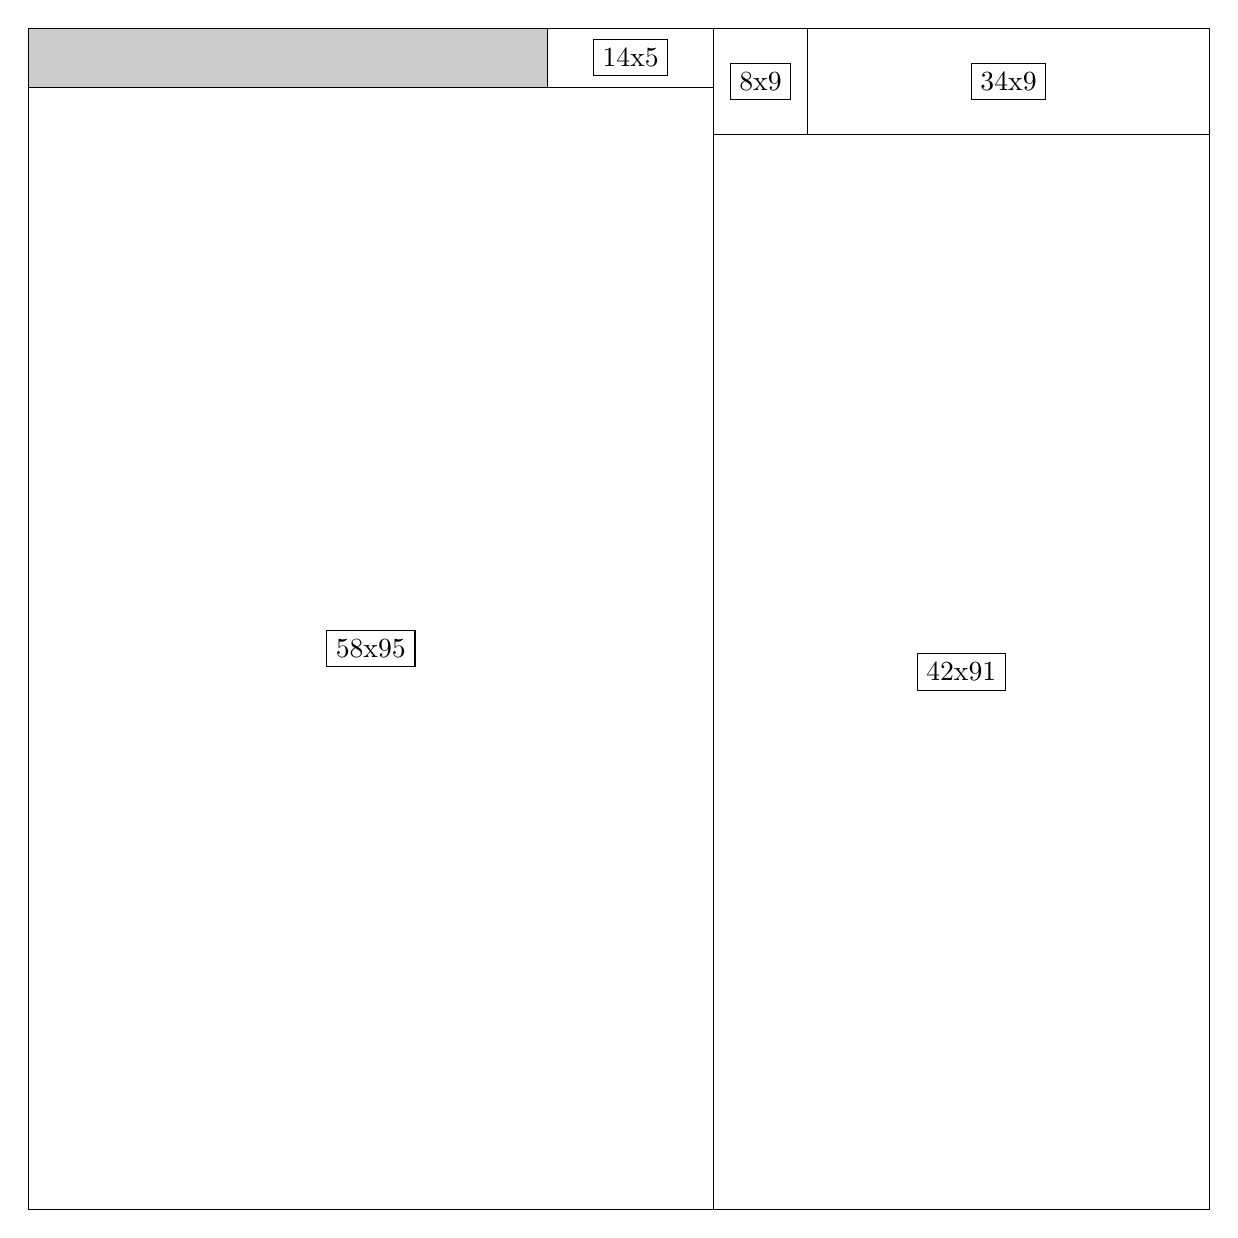
\begin{tikzpicture}[shorten >=1pt,scale=1.0,every node/.style={scale=1.0},->]
\tikzstyle{vertex}=[circle,fill=black!25,minimum size=14pt,inner sep=0pt]
\filldraw[fill=gray!40!white, draw=black] (0,0) rectangle (15.0,15.0);
\foreach \name/\x/\y/\w/\h in {58x95/0.0/0.0/8.7/14.25,42x91/8.7/0.0/6.3/13.65,34x9/9.9/13.65/5.1/1.3499999999999999,8x9/8.7/13.65/1.2/1.3499999999999999,14x5/6.6/14.25/2.1/0.75}
\filldraw[fill=white!40!white, draw=black] (\x,\y) rectangle node[draw] (\name) {\name} ++(\w,\h);
\end{tikzpicture}


w =58 , h =95 , x =0 , y =0 , v =5510
\par
w =42 , h =91 , x =58 , y =0 , v =3822
\par
w =34 , h =9 , x =66 , y =91 , v =306
\par
w =8 , h =9 , x =58 , y =91 , v =72
\par
w =14 , h =5 , x =44 , y =95 , v =70
\par
\newpage


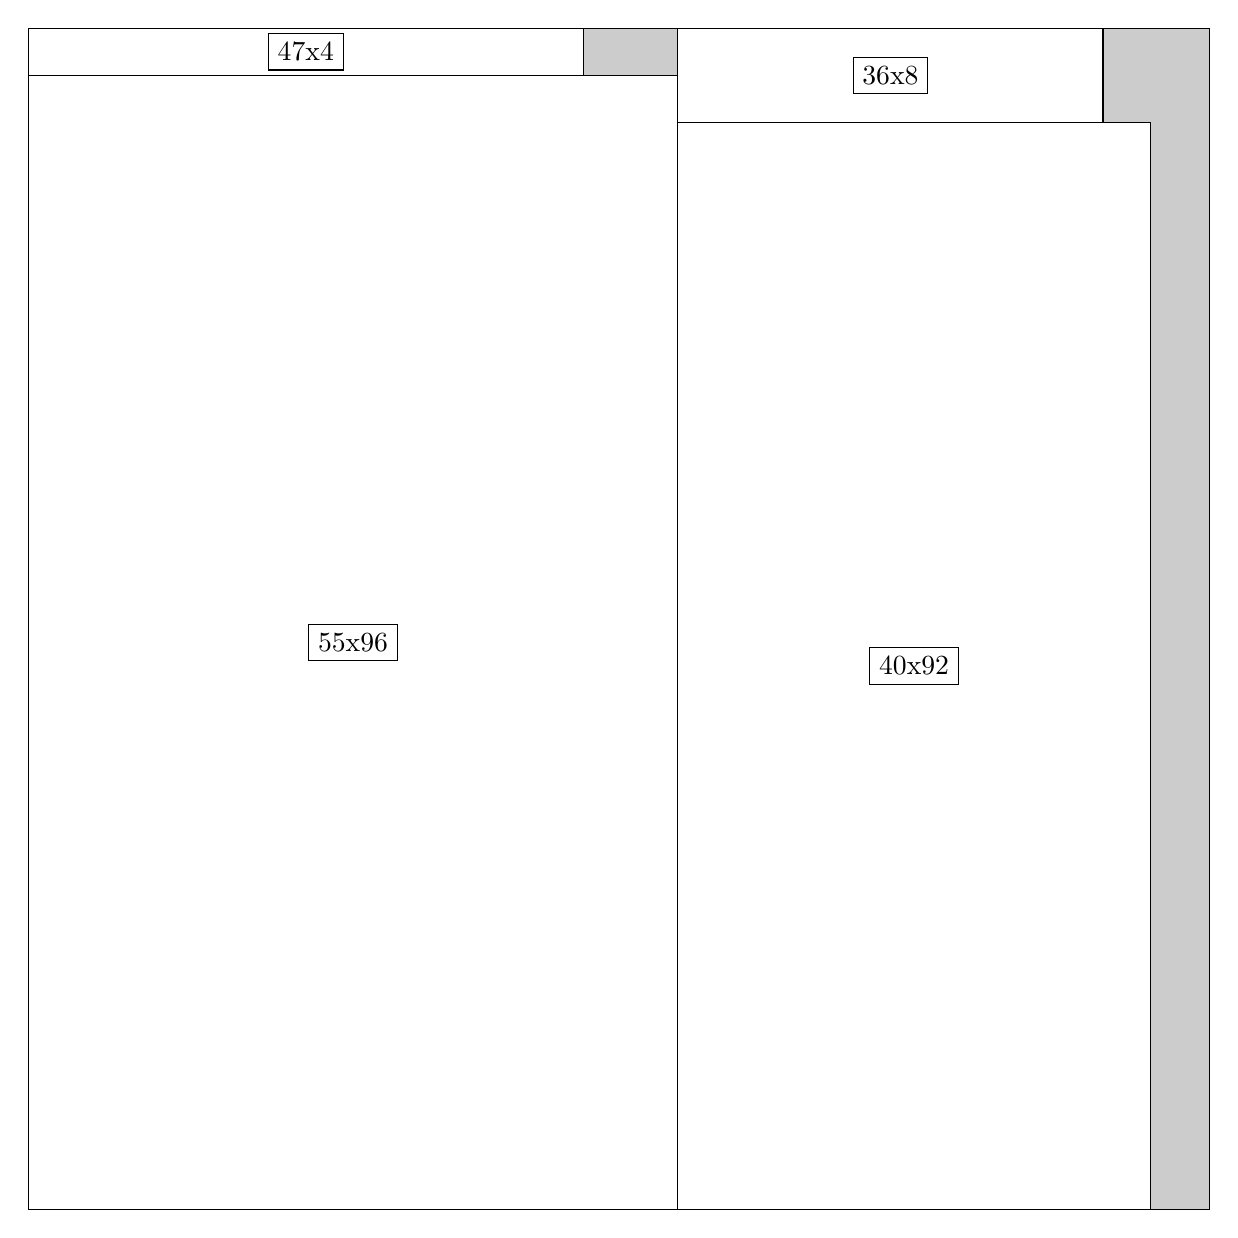
\begin{tikzpicture}[shorten >=1pt,scale=1.0,every node/.style={scale=1.0},->]
\tikzstyle{vertex}=[circle,fill=black!25,minimum size=14pt,inner sep=0pt]
\filldraw[fill=gray!40!white, draw=black] (0,0) rectangle (15.0,15.0);
\foreach \name/\x/\y/\w/\h in {55x96/0.0/0.0/8.25/14.399999999999999,40x92/8.25/0.0/6.0/13.799999999999999,36x8/8.25/13.799999999999999/5.3999999999999995/1.2,47x4/0.0/14.399999999999999/7.05/0.6}
\filldraw[fill=white!40!white, draw=black] (\x,\y) rectangle node[draw] (\name) {\name} ++(\w,\h);
\end{tikzpicture}


w =55 , h =96 , x =0 , y =0 , v =5280
\par
w =40 , h =92 , x =55 , y =0 , v =3680
\par
w =36 , h =8 , x =55 , y =92 , v =288
\par
w =47 , h =4 , x =0 , y =96 , v =188
\par
\newpage


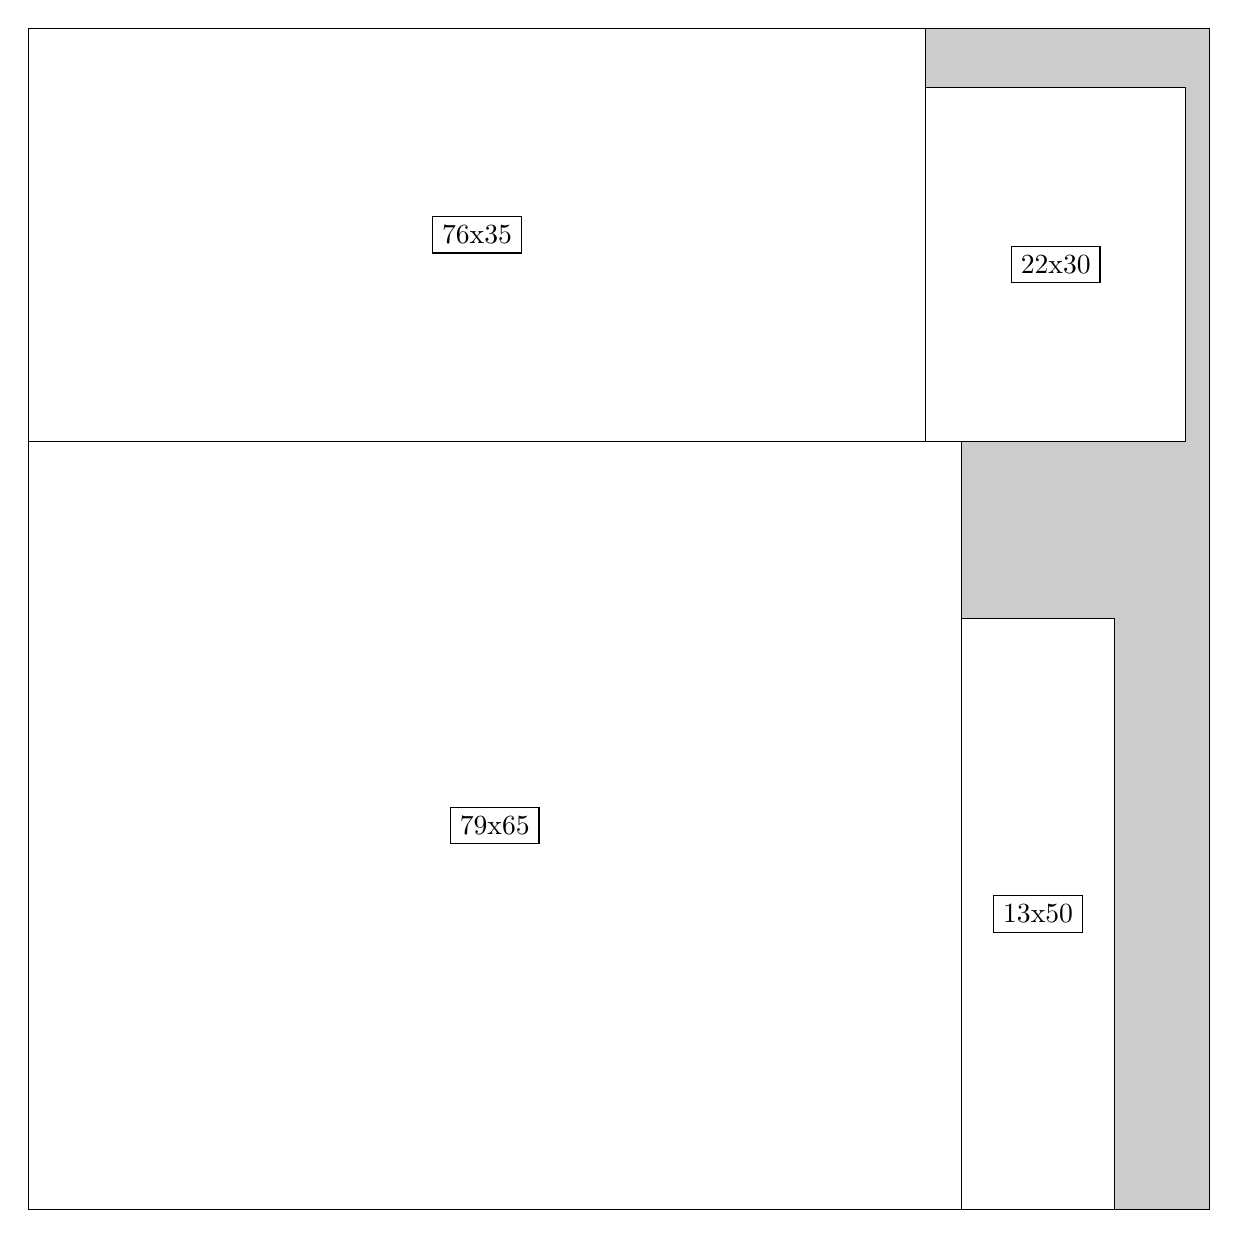
\begin{tikzpicture}[shorten >=1pt,scale=1.0,every node/.style={scale=1.0},->]
\tikzstyle{vertex}=[circle,fill=black!25,minimum size=14pt,inner sep=0pt]
\filldraw[fill=gray!40!white, draw=black] (0,0) rectangle (15.0,15.0);
\foreach \name/\x/\y/\w/\h in {79x65/0.0/0.0/11.85/9.75,76x35/0.0/9.75/11.4/5.25,13x50/11.85/0.0/1.95/7.5,22x30/11.4/9.75/3.3/4.5}
\filldraw[fill=white!40!white, draw=black] (\x,\y) rectangle node[draw] (\name) {\name} ++(\w,\h);
\end{tikzpicture}


w =79 , h =65 , x =0 , y =0 , v =5135
\par
w =76 , h =35 , x =0 , y =65 , v =2660
\par
w =13 , h =50 , x =79 , y =0 , v =650
\par
w =22 , h =30 , x =76 , y =65 , v =660
\par
\newpage


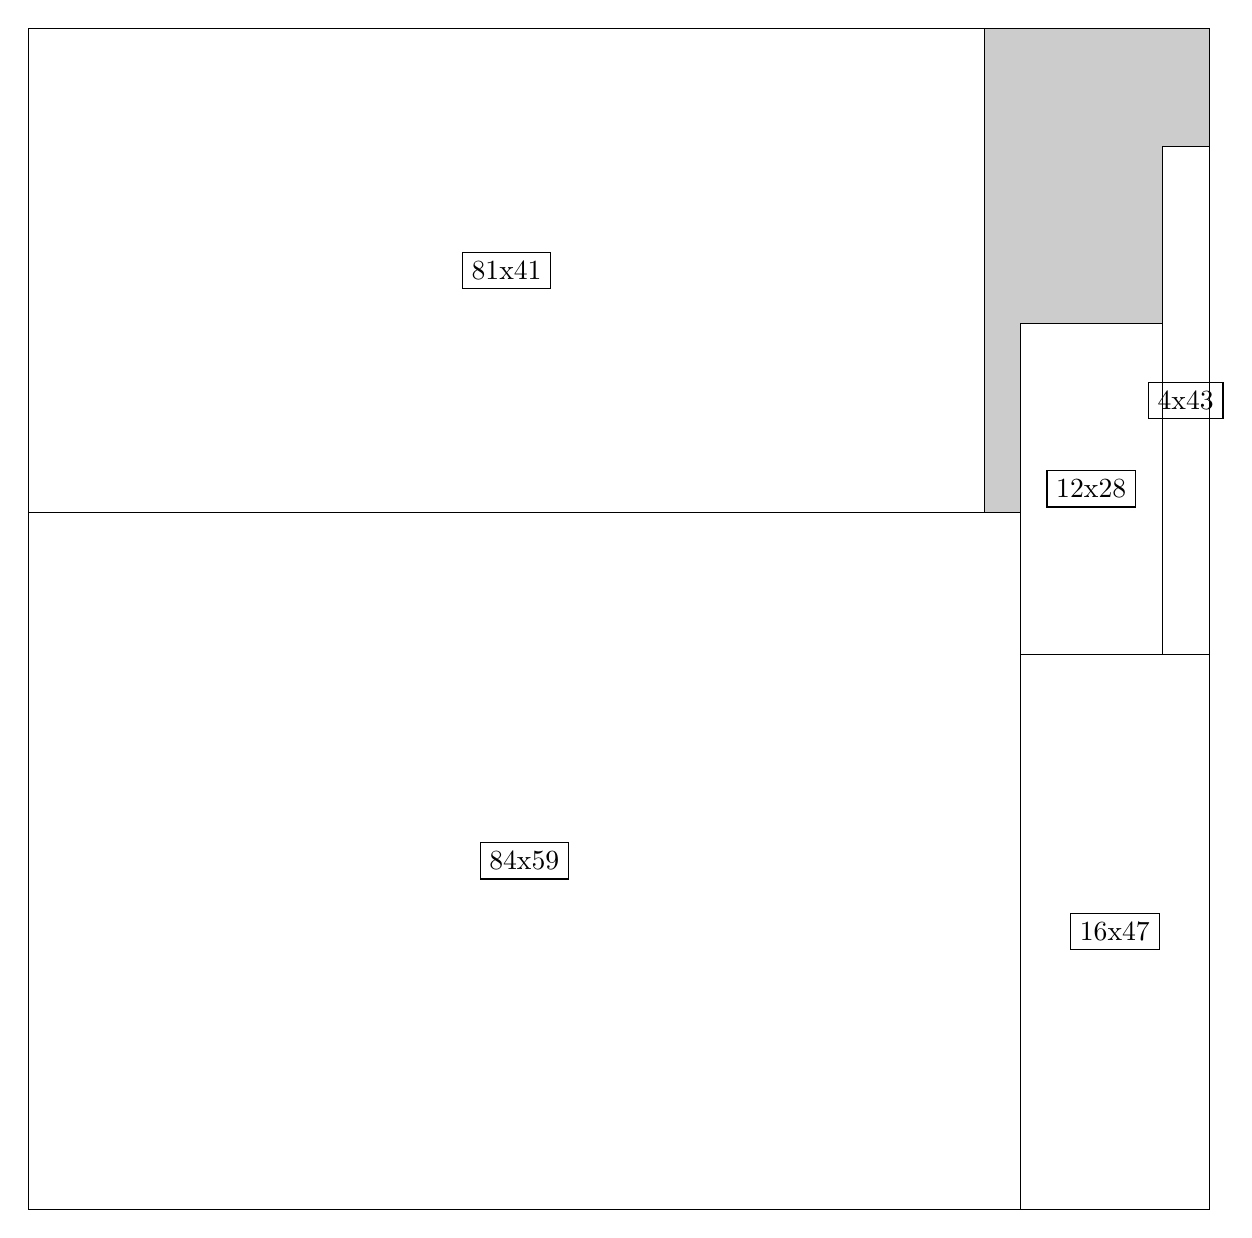
\begin{tikzpicture}[shorten >=1pt,scale=1.0,every node/.style={scale=1.0},->]
\tikzstyle{vertex}=[circle,fill=black!25,minimum size=14pt,inner sep=0pt]
\filldraw[fill=gray!40!white, draw=black] (0,0) rectangle (15.0,15.0);
\foreach \name/\x/\y/\w/\h in {84x59/0.0/0.0/12.6/8.85,81x41/0.0/8.85/12.15/6.1499999999999995,16x47/12.6/0.0/2.4/7.05,12x28/12.6/7.05/1.7999999999999998/4.2,4x43/14.399999999999999/7.05/0.6/6.45}
\filldraw[fill=white!40!white, draw=black] (\x,\y) rectangle node[draw] (\name) {\name} ++(\w,\h);
\end{tikzpicture}


w =84 , h =59 , x =0 , y =0 , v =4956
\par
w =81 , h =41 , x =0 , y =59 , v =3321
\par
w =16 , h =47 , x =84 , y =0 , v =752
\par
w =12 , h =28 , x =84 , y =47 , v =336
\par
w =4 , h =43 , x =96 , y =47 , v =172
\par
\newpage


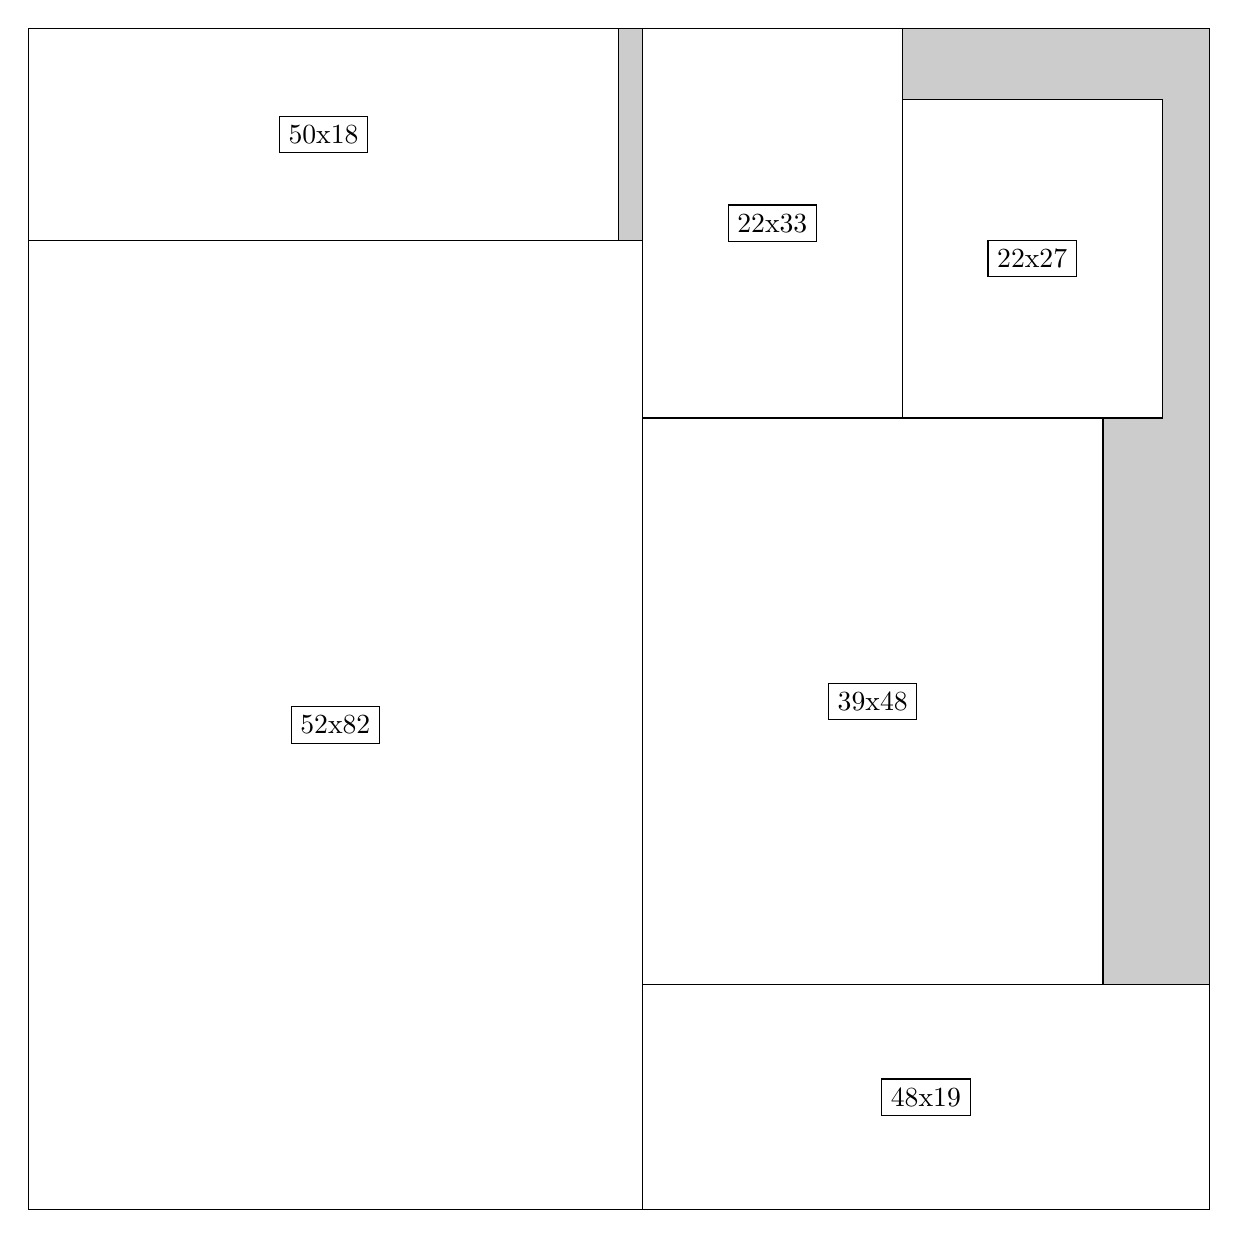
\begin{tikzpicture}[shorten >=1pt,scale=1.0,every node/.style={scale=1.0},->]
\tikzstyle{vertex}=[circle,fill=black!25,minimum size=14pt,inner sep=0pt]
\filldraw[fill=gray!40!white, draw=black] (0,0) rectangle (15.0,15.0);
\foreach \name/\x/\y/\w/\h in {52x82/0.0/0.0/7.8/12.299999999999999,48x19/7.8/0.0/7.199999999999999/2.85,39x48/7.8/2.85/5.85/7.199999999999999,50x18/0.0/12.299999999999999/7.5/2.6999999999999997,22x33/7.8/10.049999999999999/3.3/4.95,22x27/11.1/10.049999999999999/3.3/4.05}
\filldraw[fill=white!40!white, draw=black] (\x,\y) rectangle node[draw] (\name) {\name} ++(\w,\h);
\end{tikzpicture}


w =52 , h =82 , x =0 , y =0 , v =4264
\par
w =48 , h =19 , x =52 , y =0 , v =912
\par
w =39 , h =48 , x =52 , y =19 , v =1872
\par
w =50 , h =18 , x =0 , y =82 , v =900
\par
w =22 , h =33 , x =52 , y =67 , v =726
\par
w =22 , h =27 , x =74 , y =67 , v =594
\par
\newpage


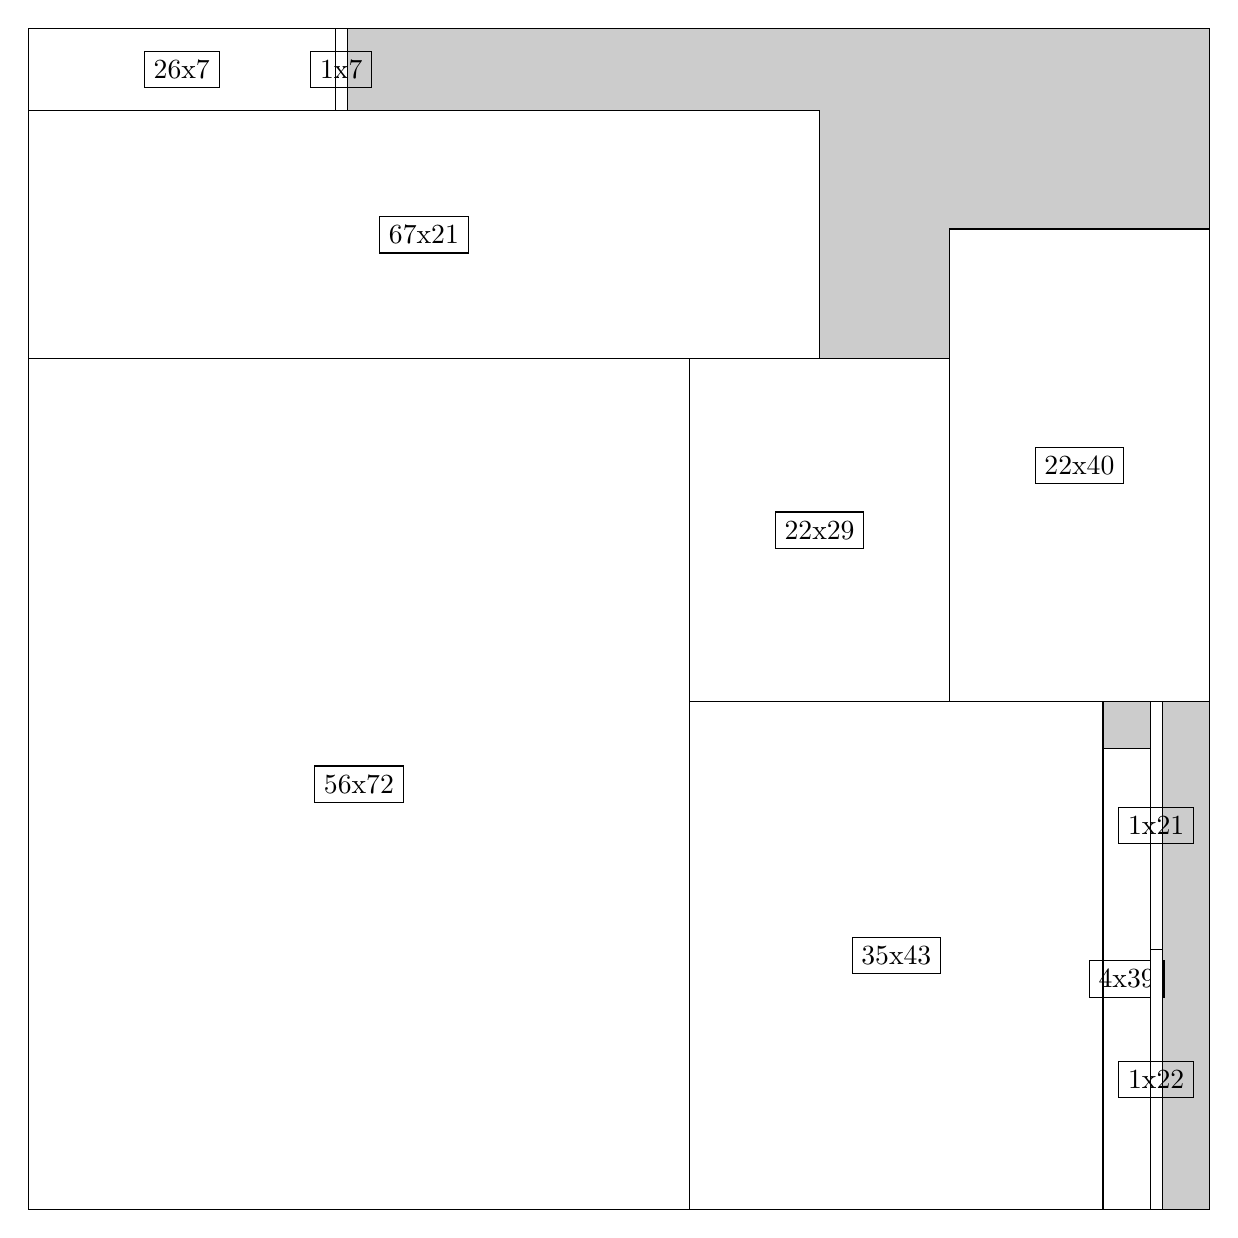
\begin{tikzpicture}[shorten >=1pt,scale=1.0,every node/.style={scale=1.0},->]
\tikzstyle{vertex}=[circle,fill=black!25,minimum size=14pt,inner sep=0pt]
\filldraw[fill=gray!40!white, draw=black] (0,0) rectangle (15.0,15.0);
\foreach \name/\x/\y/\w/\h in {56x72/0.0/0.0/8.4/10.799999999999999,35x43/8.4/0.0/5.25/6.45,67x21/0.0/10.799999999999999/10.049999999999999/3.15,22x40/11.7/6.45/3.3/6.0,22x29/8.4/6.45/3.3/4.35,26x7/0.0/13.95/3.9/1.05,4x39/13.65/0.0/0.6/5.85,1x22/14.25/0.0/0.15/3.3,1x21/14.25/3.3/0.15/3.15,1x7/3.9/13.95/0.15/1.05}
\filldraw[fill=white!40!white, draw=black] (\x,\y) rectangle node[draw] (\name) {\name} ++(\w,\h);
\end{tikzpicture}


w =56 , h =72 , x =0 , y =0 , v =4032
\par
w =35 , h =43 , x =56 , y =0 , v =1505
\par
w =67 , h =21 , x =0 , y =72 , v =1407
\par
w =22 , h =40 , x =78 , y =43 , v =880
\par
w =22 , h =29 , x =56 , y =43 , v =638
\par
w =26 , h =7 , x =0 , y =93 , v =182
\par
w =4 , h =39 , x =91 , y =0 , v =156
\par
w =1 , h =22 , x =95 , y =0 , v =22
\par
w =1 , h =21 , x =95 , y =22 , v =21
\par
w =1 , h =7 , x =26 , y =93 , v =7
\par
\newpage


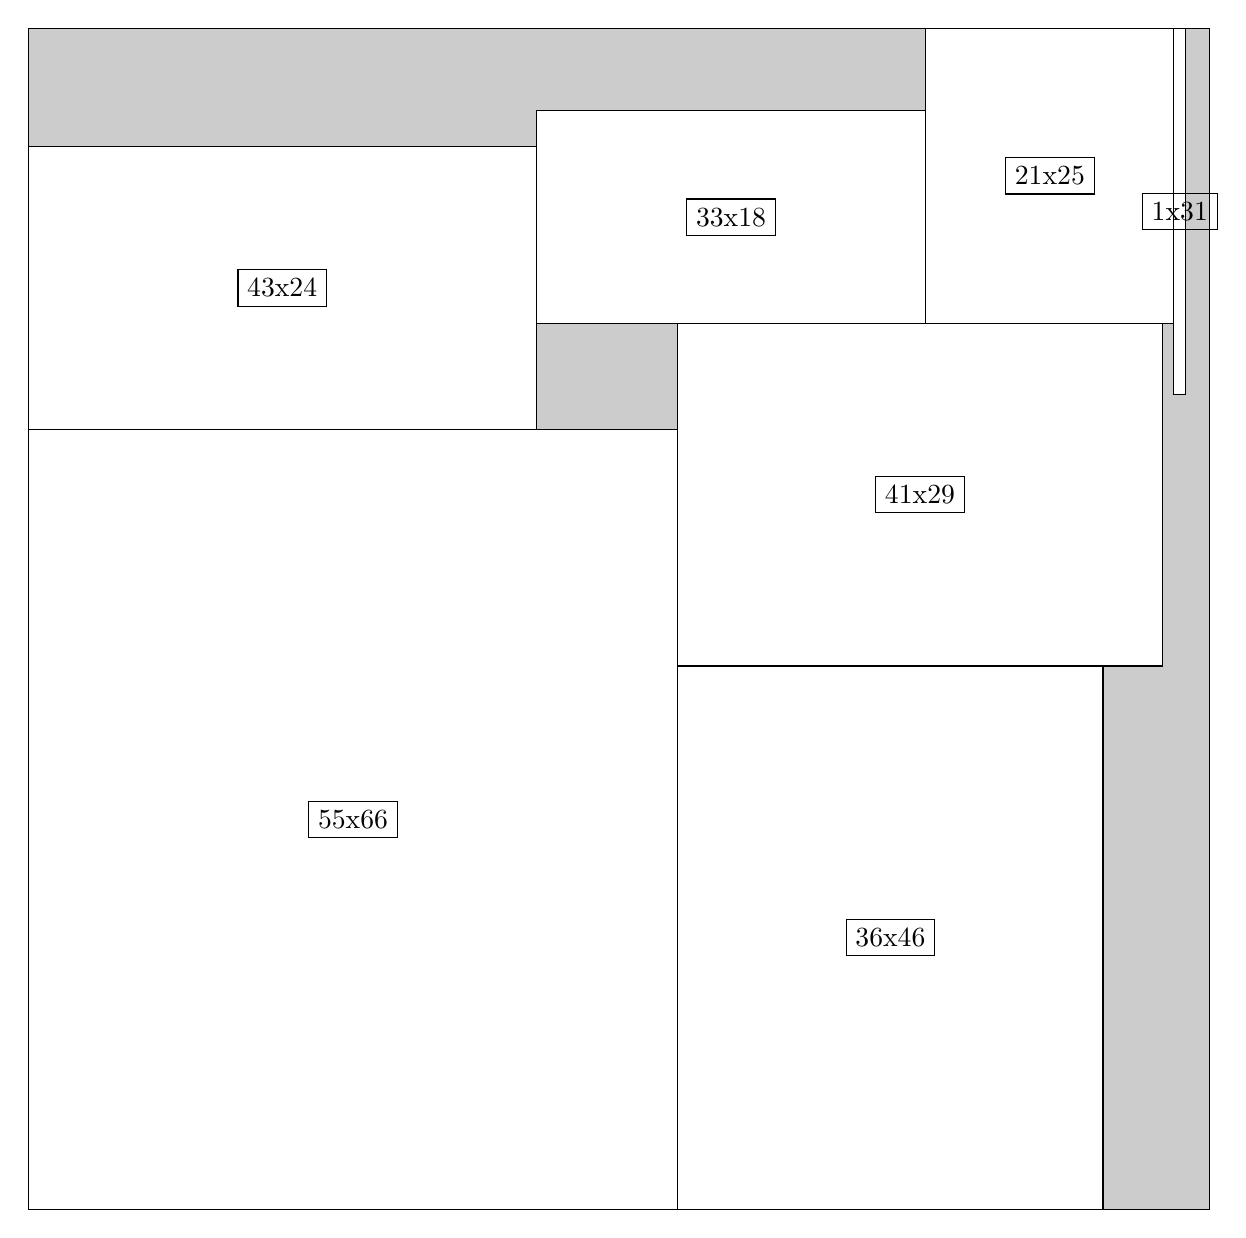
\begin{tikzpicture}[shorten >=1pt,scale=1.0,every node/.style={scale=1.0},->]
\tikzstyle{vertex}=[circle,fill=black!25,minimum size=14pt,inner sep=0pt]
\filldraw[fill=gray!40!white, draw=black] (0,0) rectangle (15.0,15.0);
\foreach \name/\x/\y/\w/\h in {43x24/0.0/9.9/6.45/3.5999999999999996,36x46/8.25/0.0/5.3999999999999995/6.8999999999999995,41x29/8.25/6.8999999999999995/6.1499999999999995/4.35,55x66/0.0/0.0/8.25/9.9,33x18/6.45/11.25/4.95/2.6999999999999997,21x25/11.4/11.25/3.15/3.75,1x31/14.549999999999999/10.35/0.15/4.6499999999999995}
\filldraw[fill=white!40!white, draw=black] (\x,\y) rectangle node[draw] (\name) {\name} ++(\w,\h);
\end{tikzpicture}


w =43 , h =24 , x =0 , y =66 , v =1032
\par
w =36 , h =46 , x =55 , y =0 , v =1656
\par
w =41 , h =29 , x =55 , y =46 , v =1189
\par
w =55 , h =66 , x =0 , y =0 , v =3630
\par
w =33 , h =18 , x =43 , y =75 , v =594
\par
w =21 , h =25 , x =76 , y =75 , v =525
\par
w =1 , h =31 , x =97 , y =69 , v =31
\par
\newpage


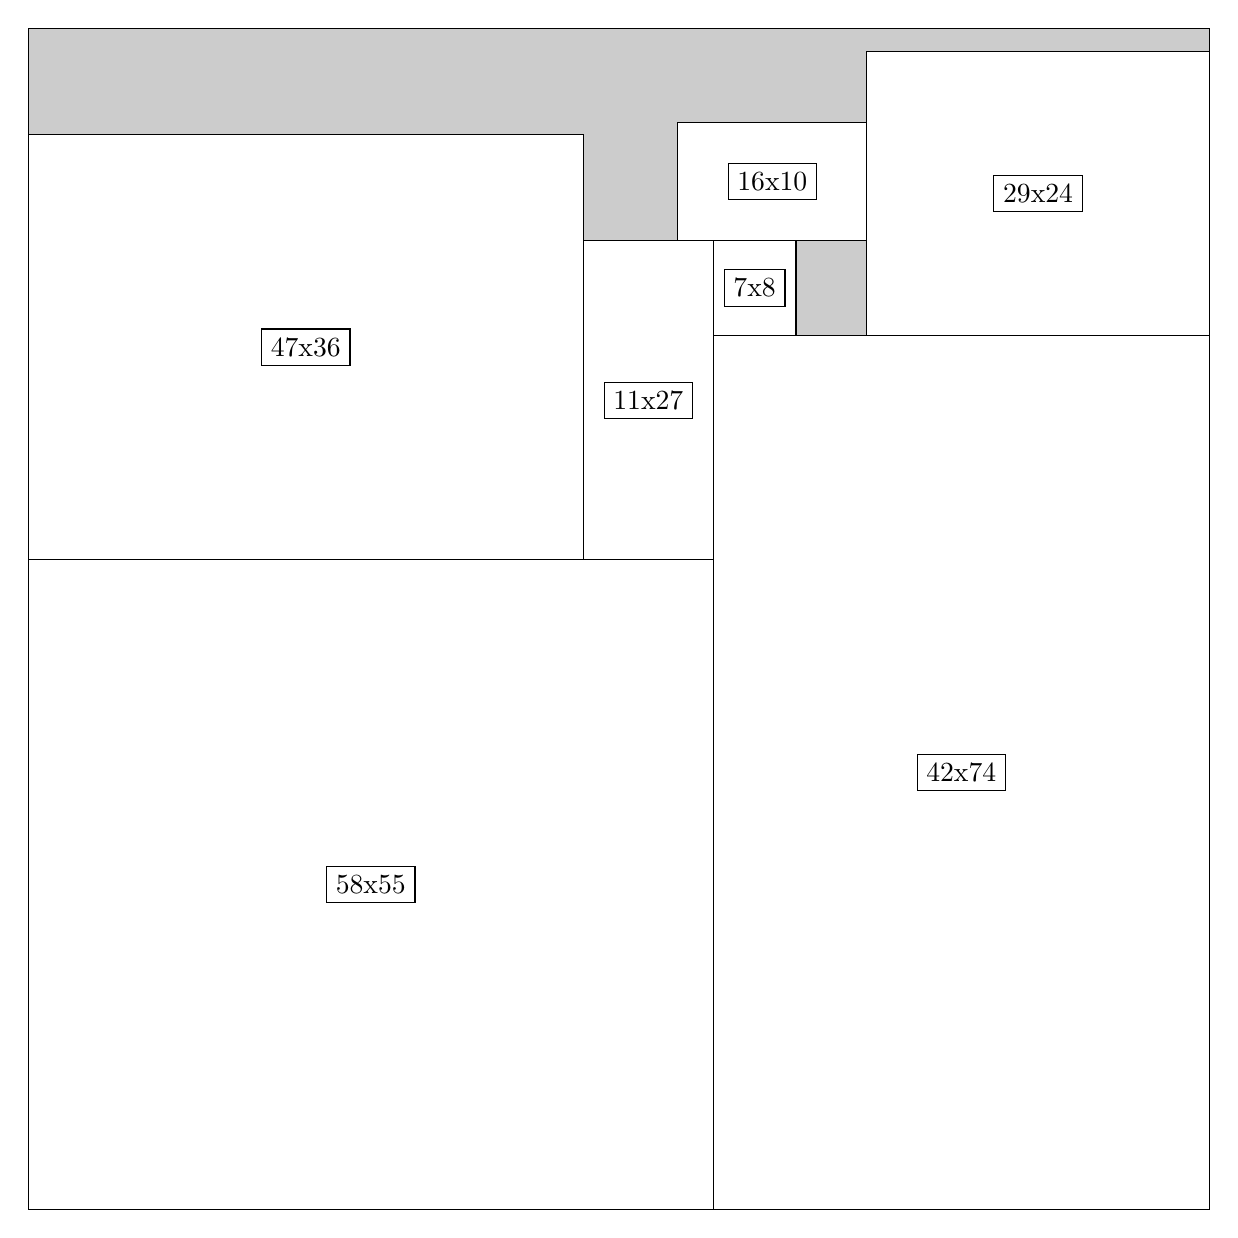
\begin{tikzpicture}[shorten >=1pt,scale=1.0,every node/.style={scale=1.0},->]
\tikzstyle{vertex}=[circle,fill=black!25,minimum size=14pt,inner sep=0pt]
\filldraw[fill=gray!40!white, draw=black] (0,0) rectangle (15.0,15.0);
\foreach \name/\x/\y/\w/\h in {58x55/0.0/0.0/8.7/8.25,42x74/8.7/0.0/6.3/11.1,47x36/0.0/8.25/7.05/5.3999999999999995,7x8/8.7/11.1/1.05/1.2,29x24/10.65/11.1/4.35/3.5999999999999996,11x27/7.05/8.25/1.65/4.05,16x10/8.25/12.299999999999999/2.4/1.5}
\filldraw[fill=white!40!white, draw=black] (\x,\y) rectangle node[draw] (\name) {\name} ++(\w,\h);
\end{tikzpicture}


w =58 , h =55 , x =0 , y =0 , v =3190
\par
w =42 , h =74 , x =58 , y =0 , v =3108
\par
w =47 , h =36 , x =0 , y =55 , v =1692
\par
w =7 , h =8 , x =58 , y =74 , v =56
\par
w =29 , h =24 , x =71 , y =74 , v =696
\par
w =11 , h =27 , x =47 , y =55 , v =297
\par
w =16 , h =10 , x =55 , y =82 , v =160
\par
\newpage


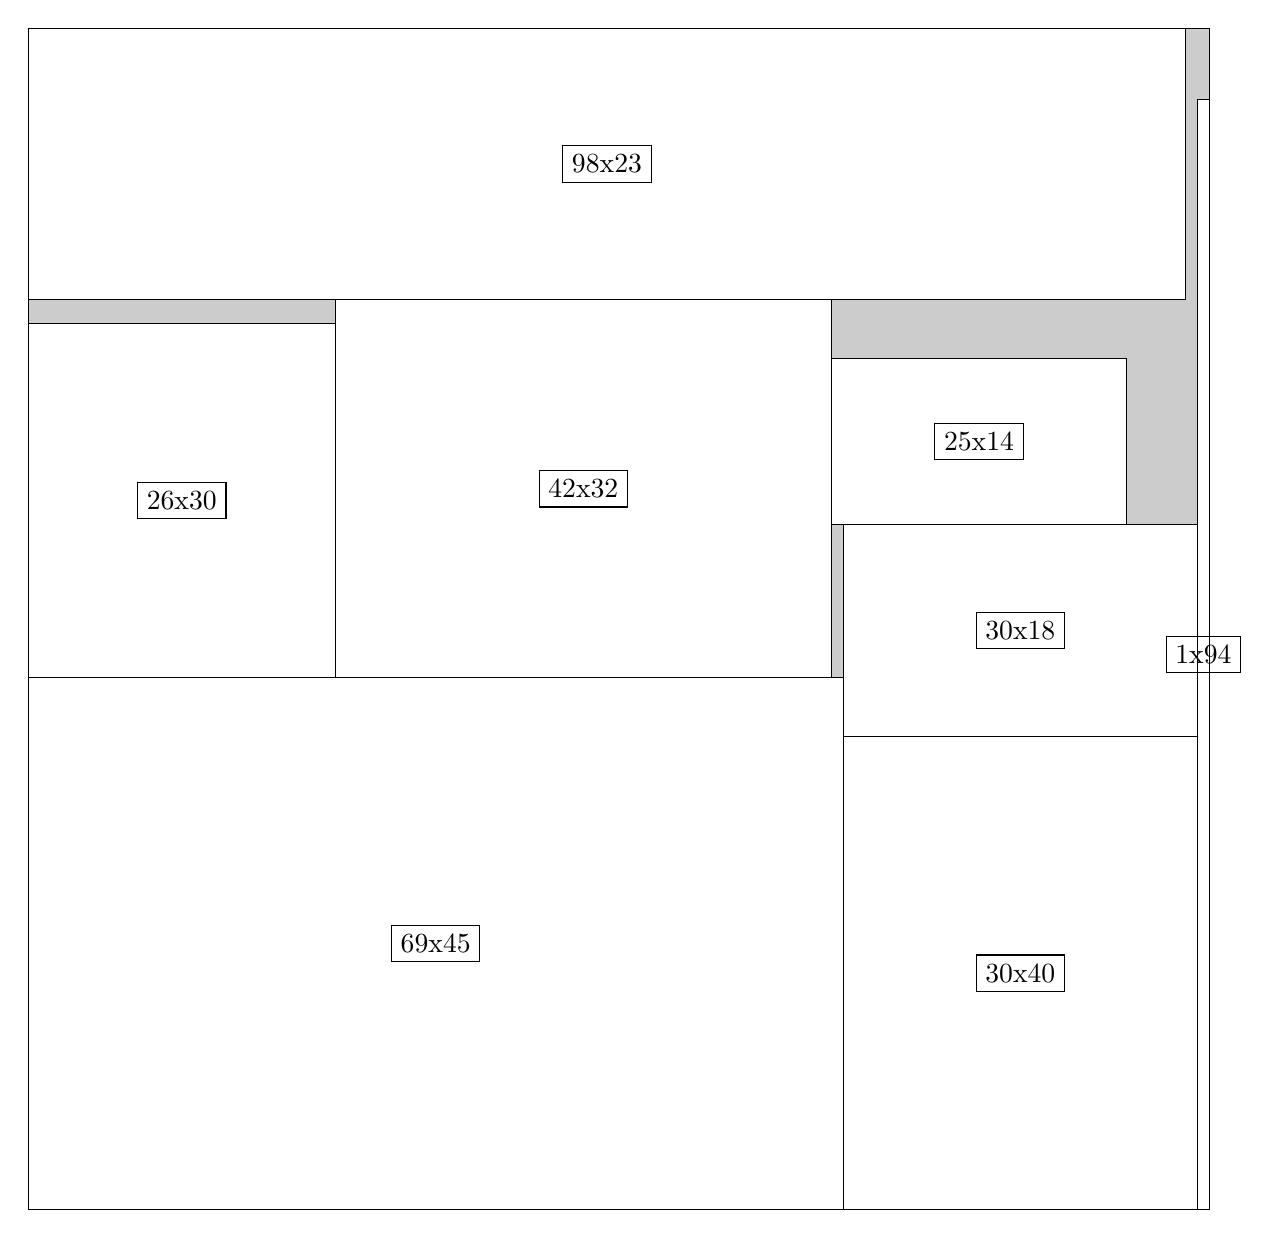
\begin{tikzpicture}[shorten >=1pt,scale=1.0,every node/.style={scale=1.0},->]
\tikzstyle{vertex}=[circle,fill=black!25,minimum size=14pt,inner sep=0pt]
\filldraw[fill=gray!40!white, draw=black] (0,0) rectangle (15.0,15.0);
\foreach \name/\x/\y/\w/\h in {69x45/0.0/0.0/10.35/6.75,98x23/0.0/11.549999999999999/14.7/3.4499999999999997,30x40/10.35/0.0/4.5/6.0,26x30/0.0/6.75/3.9/4.5,30x18/10.35/6.0/4.5/2.6999999999999997,25x14/10.2/8.7/3.75/2.1,1x94/14.85/0.0/0.15/14.1,42x32/3.9/6.75/6.3/4.8}
\filldraw[fill=white!40!white, draw=black] (\x,\y) rectangle node[draw] (\name) {\name} ++(\w,\h);
\end{tikzpicture}


w =69 , h =45 , x =0 , y =0 , v =3105
\par
w =98 , h =23 , x =0 , y =77 , v =2254
\par
w =30 , h =40 , x =69 , y =0 , v =1200
\par
w =26 , h =30 , x =0 , y =45 , v =780
\par
w =30 , h =18 , x =69 , y =40 , v =540
\par
w =25 , h =14 , x =68 , y =58 , v =350
\par
w =1 , h =94 , x =99 , y =0 , v =94
\par
w =42 , h =32 , x =26 , y =45 , v =1344
\par
\newpage


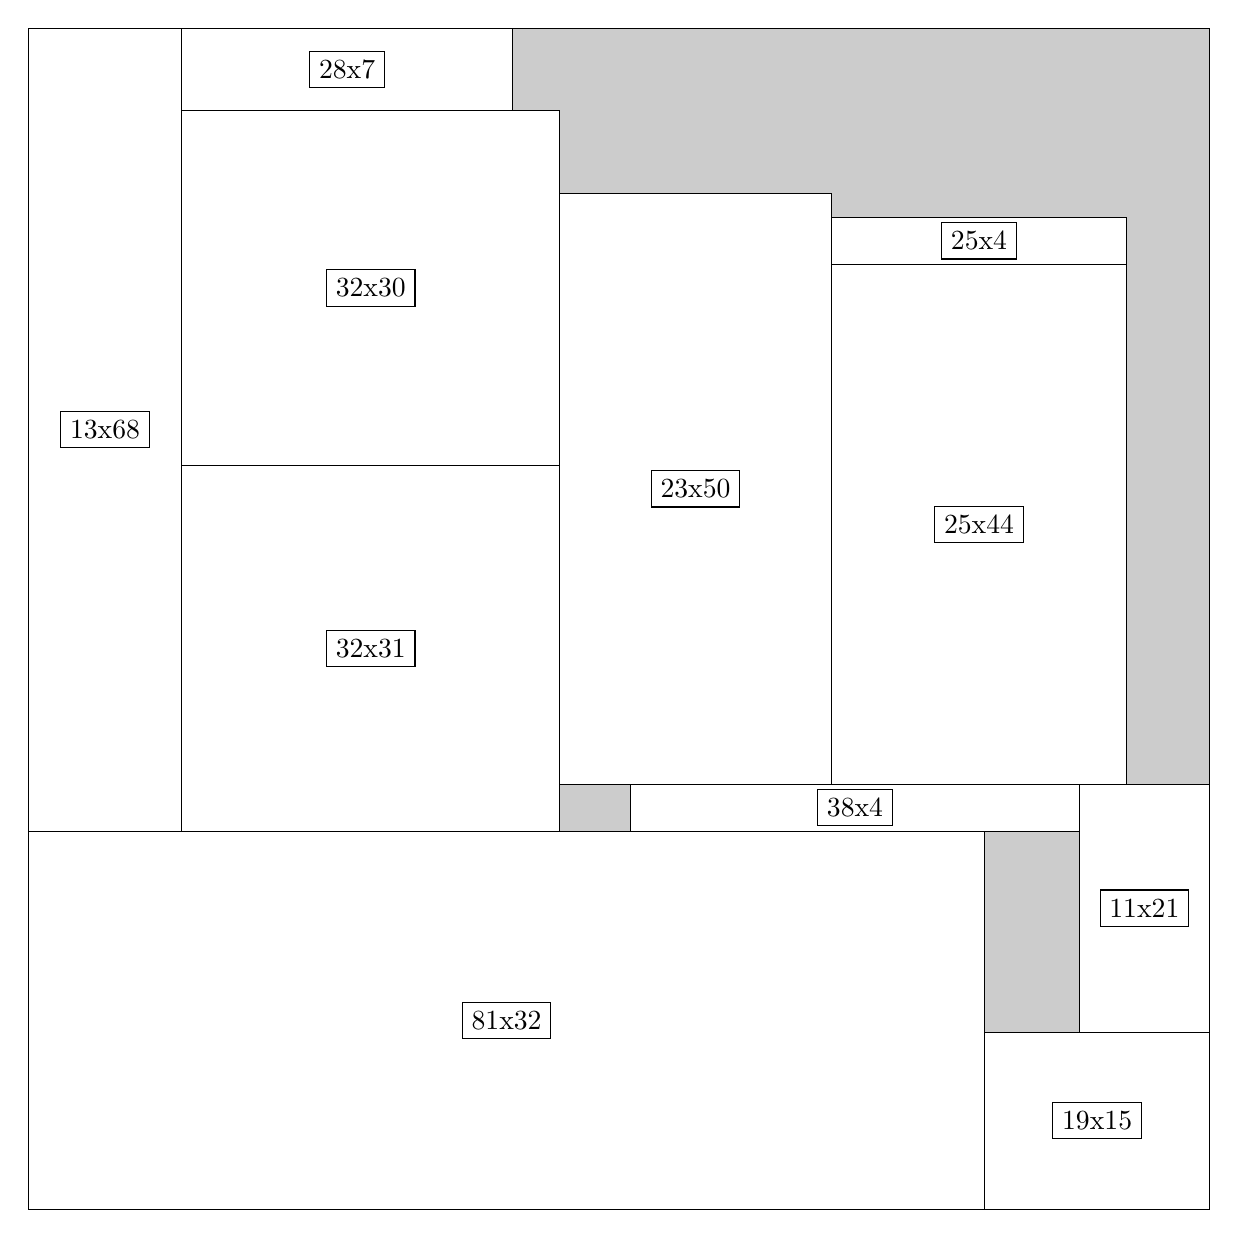
\begin{tikzpicture}[shorten >=1pt,scale=1.0,every node/.style={scale=1.0},->]
\tikzstyle{vertex}=[circle,fill=black!25,minimum size=14pt,inner sep=0pt]
\filldraw[fill=gray!40!white, draw=black] (0,0) rectangle (15.0,15.0);
\foreach \name/\x/\y/\w/\h in {81x32/0.0/0.0/12.15/4.8,23x50/6.75/5.3999999999999995/3.4499999999999997/7.5,25x44/10.2/5.3999999999999995/3.75/6.6,32x31/1.95/4.8/4.8/4.6499999999999995,32x30/1.95/9.45/4.8/4.5,13x68/0.0/4.8/1.95/10.2,19x15/12.15/0.0/2.85/2.25,11x21/13.35/2.25/1.65/3.15,28x7/1.95/13.95/4.2/1.05,38x4/7.6499999999999995/4.8/5.7/0.6,25x4/10.2/12.0/3.75/0.6}
\filldraw[fill=white!40!white, draw=black] (\x,\y) rectangle node[draw] (\name) {\name} ++(\w,\h);
\end{tikzpicture}


w =81 , h =32 , x =0 , y =0 , v =2592
\par
w =23 , h =50 , x =45 , y =36 , v =1150
\par
w =25 , h =44 , x =68 , y =36 , v =1100
\par
w =32 , h =31 , x =13 , y =32 , v =992
\par
w =32 , h =30 , x =13 , y =63 , v =960
\par
w =13 , h =68 , x =0 , y =32 , v =884
\par
w =19 , h =15 , x =81 , y =0 , v =285
\par
w =11 , h =21 , x =89 , y =15 , v =231
\par
w =28 , h =7 , x =13 , y =93 , v =196
\par
w =38 , h =4 , x =51 , y =32 , v =152
\par
w =25 , h =4 , x =68 , y =80 , v =100
\par
\newpage


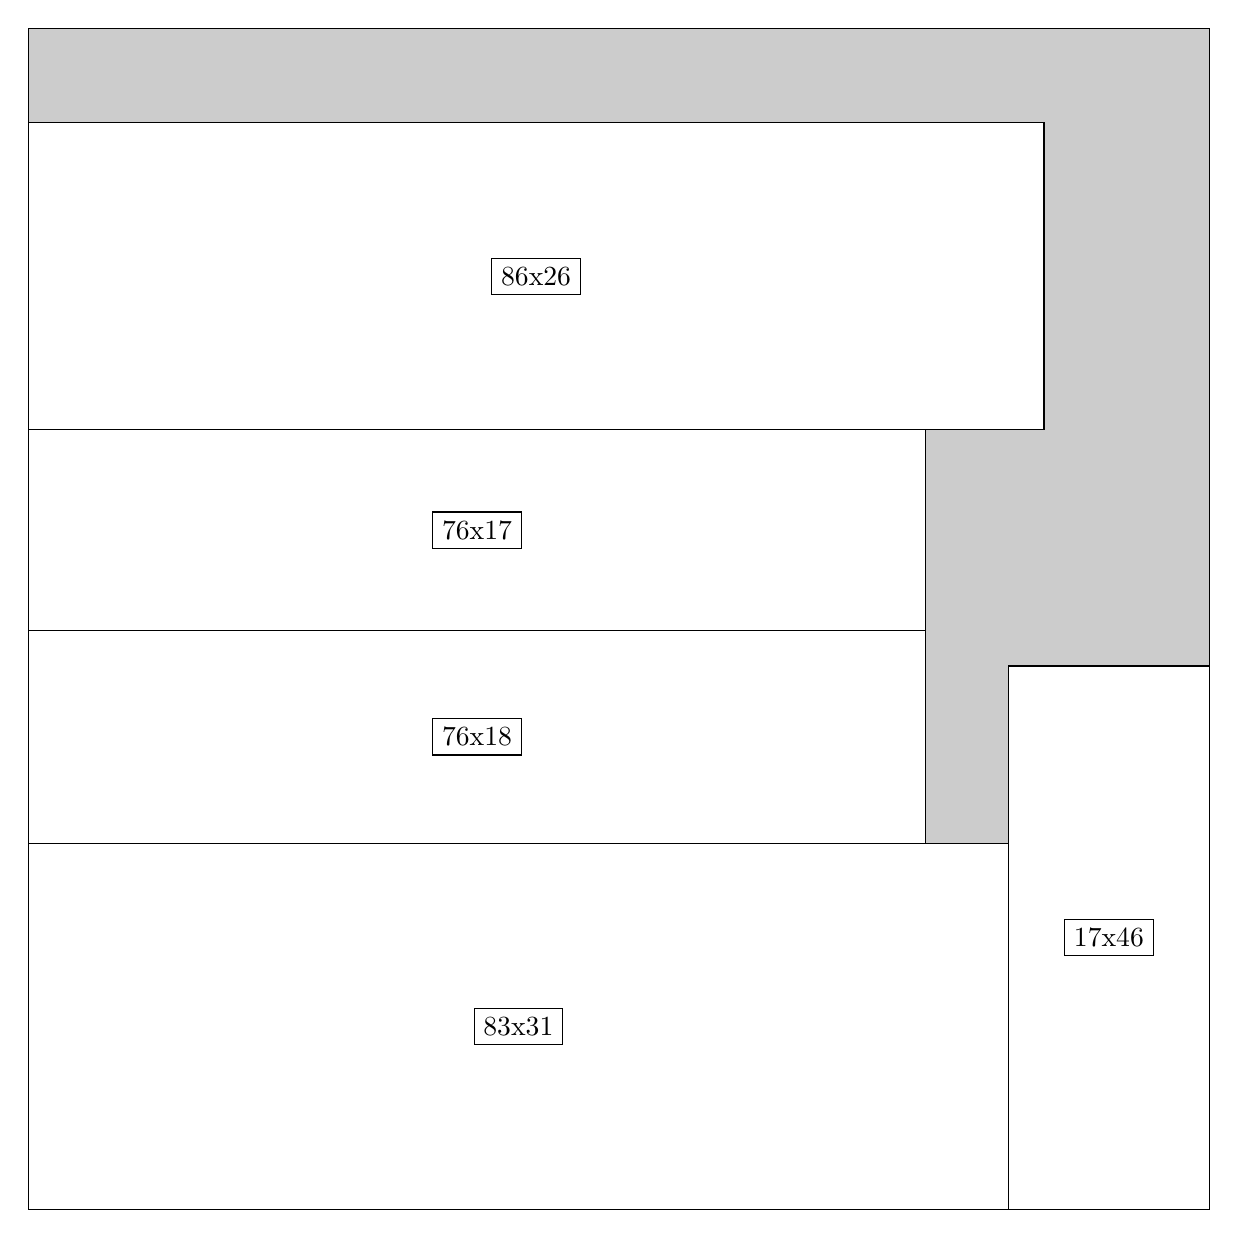
\begin{tikzpicture}[shorten >=1pt,scale=1.0,every node/.style={scale=1.0},->]
\tikzstyle{vertex}=[circle,fill=black!25,minimum size=14pt,inner sep=0pt]
\filldraw[fill=gray!40!white, draw=black] (0,0) rectangle (15.0,15.0);
\foreach \name/\x/\y/\w/\h in {83x31/0.0/0.0/12.45/4.6499999999999995,86x26/0.0/9.9/12.9/3.9,76x18/0.0/4.6499999999999995/11.4/2.6999999999999997,76x17/0.0/7.35/11.4/2.55,17x46/12.45/0.0/2.55/6.8999999999999995}
\filldraw[fill=white!40!white, draw=black] (\x,\y) rectangle node[draw] (\name) {\name} ++(\w,\h);
\end{tikzpicture}


w =83 , h =31 , x =0 , y =0 , v =2573
\par
w =86 , h =26 , x =0 , y =66 , v =2236
\par
w =76 , h =18 , x =0 , y =31 , v =1368
\par
w =76 , h =17 , x =0 , y =49 , v =1292
\par
w =17 , h =46 , x =83 , y =0 , v =782
\par
\newpage


\end{document}